% To je predloga za poročilo projekta pripredmetu Osnove verjetnosti in
% statistike.
% Originalen avtor predloge je Blaž Zupan.
% Za potrebe OVS je prilagodil Robert Cvitkovič
% To predlogo lahko spremeniš v PDF dokument s pomočjo programa
% pdflatex, ki je del standardne instalacije LaTeX programov.

\documentclass[a4paper,11pt]{article}
\usepackage[utf8]{inputenc}
\usepackage{amsmath, amssymb, amsthm, amsfonts, mathtools}
\usepackage{a4wide}
\usepackage[slovene]{babel}
\usepackage{graphicx}
\usepackage{url}
\usepackage{float}
\usepackage[pdftex,pdfpagelabels,bookmarks,hyperindex,hyperfigures]{hyperref}
% \usepackage{hyperref}
\hypersetup{
pdffitwindow=true,              % window fit to page when opened
pdftitle={Seminarska pri predmetu VIS},       % title
pdfauthor={Matej Kalc},                % author
pdfnewwindow=true,              % links in new window
colorlinks=true,                % false: boxed links; true: colored links
linkcolor=blue,                 % color of internal links
citecolor=blue,                 % color of links to bibliography
filecolor=blue,                 % color of file links
urlcolor=cyan                   % color of external links
}

% \usepackage{tikz}
% \usepackage{pgflibraryshapes}

\usepackage[footnotesize,labelfont=bf,labelsep=period]{caption}
\usepackage{enumerate}
\usepackage{pdfpages}
\usepackage{csvsimple}

\begin{filecontents*}{db.csv}
DR,KOD,MED,DPO,DPS,DVO,DVS,OV,MV,PREB,OTO,OTS
Austria,AT,44.0,2020-02-25,2020-03-12,2020-03-27,2020-04-23,7029,52,9025715,38809,201454
Belgium,BE,41.4,2020-02-04,2020-03-10,2020-04-11,2020-04-12,32778,4273,11602522,103714,109427
Bulgaria,BG,42.7,2020-03-08,2020-03-12,2020-06-12,2020-06-06,3086,168,6943915,91083,81084
Croatia,HR,43.0,2020-02-25,2020-03-25,2020-04-02,2020-04-20,963,6,4101782,8110,25566
Cyprus,CY,36.8,2020-03-09,2020-03-25,2020-04-02,2020-03-25,320,9,1190007,8468,3849
Czechia,CZ,42.1,2020-03-01,2020-03-23,2020-03-27,2020-04-15,2062,9,10715154,36089,148586
Denmark,DK,42.2,2020-02-27,2020-03-15,2020-04-08,2020-04-05,5071,203,5793679,62063,50097
Estonia,EE,42.7,2020-02-27,2020-03-26,2020-03-27,2020-04-03,538,1,1328655,9010,18172
Finland,FI,42.5,2020-01-29,2020-03-21,2020-04-05,2020-04-22,1882,25,5542713,34486,76173
France,FR,41.4,2020-01-24,2020-02-15,2020-04-01,2020-04-04,51477,3514,65283211,233494,282205
Germany,DE,47.1,2020-01-28,2020-03-09,2020-03-20,2020-04-16,18323,45,83951077,595836,2019592
Greece,GR,44.5,2020-02-26,2020-03-12,2020-04-22,2020-04-05,2401,121,10420046,58847,26200
Hungary,HU,42.3,2020-03-04,2020-03-15,2020-04-10,2020-04-24,1190,77,9659639,29041,57641
Ireland,IE,36.8,2020-03-01,2020-03-11,2020-04-10,2020-04-26,7393,263,4953657,68922,142512
Italy,IT,45.5,2020-01-29,2020-02-22,2020-03-21,2020-03-28,53578,4827,60465251,239558,428323
Latvia,LV,43.6,2020-03-02,2020-04-04,2020-03-24,2020-04-22,180,0,1883138,8281,40057
Lithuania,LT,43.7,2020-02-28,2020-03-20,2020-04-04,2020-04-12,771,9,2714541,21467,40951
Luxembourg,LU,39.3,2020-03-01,2020-03-13,2020-03-24,2020-04-12,875,8,628614,11189,29881
Malta,MT,41.8,2020-03-07,2020-04-09,2020-04-08,2020-06-02,293,0,441612,14119,73236
Netherlands,NL,42.6,2020-02-27,2020-03-06,2020-03-24,2020-04-08,4749,213,17138553,45825,109414
Poland,PL,40.7,2020-03-05,2020-03-12,2020-06-05,2020-04-25,25048,1117,37850596,1006819,271678
Portugal,PT,42.2,2020-03-02,2020-03-17,2020-04-11,2020-04-04,15472,435,10193282,179542,112892
Romania,RO,41.1,2020-02-26,2020-03-23,2020-04-12,2020-05-01,5990,282,19210031,64385,175728
Slovakia,SK,40.5,2020-03-06,2020-04-07,2020-04-17,2020-04-16,977,8,5461415,42768,40048
Slovenia,SI,44.5,2020-03-04,2020-03-17,2020-03-13,2020-04-06,141,0,2079553,4228,28453
Spain,ES,42.7,2020-01-31,2020-03-04,2020-04-01,2020-06-20,94417,8189,46785134,466271,3627852
Sweden,SE,41.2,2020-01-31,2020-03-15,2020-06-23,2020-04-22,58932,5122,10108080,467798,105806
\end{filecontents*}


\begin{filecontents*}{dbIntervalZaupanjaDelezOkuzenih.csv}
Ime drzave,Spodnja meja intervala,Zgornja meja intervala
Austria,0.076\%,0.08\%
Belgium,0.279\%,0.286\%
Bulgaria,0.043\%,0.046\%
Croatia,0.022\%,0.025\%
Cyprus,0.024\%,0.03\%
Czechia,0.018\%,0.02\%
Denmark,0.085\%,0.09\%
Estonia,0.037\%,0.044\%
Finland,0.032\%,0.036\%
France,0.078\%,0.08\%
Germany,0.022\%,0.022\%
Greece,0.022\%,0.024\%
Hungary,0.012\%,0.013\%
Ireland,0.146\%,0.153\%
Italy,0.088\%,0.089\%
Latvia,0.008\%,0.011\%
Lithuania,0.026\%,0.03\%
Luxembourg,0.13\%,0.149\%
Malta,0.059\%,0.075\%
Netherlands,0.027\%,0.029\%
Poland,0.065\%,0.067\%
Portugal,0.149\%,0.154\%
Romania,0.03\%,0.032\%
Slovakia,0.017\%,0.019\%
Slovenia,0.006\%,0.008\%
Spain,0.201\%,0.203\%
Sweden,0.578\%,0.588\%
\end{filecontents*}


\begin{filecontents*}{dbIntervalZaupanjaFatalnost.csv}
Ime drzave,Spodnja meja intervala,Zgornja meja intervala
Austria,0.558\%,0.977\%
Belgium,12.674\%,13.407\%
Bulgaria,4.682\%,6.319\%
Croatia,0.254\%,1.423\%
Cyprus,1.379\%,5.458\%
Czechia,0.213\%,0.859\%
Denmark,3.488\%,4.589\%
Estonia,0.01\%,1.198\%
Finland,0.88\%,1.985\%
France,6.611\%,7.048\%
Germany,0.181\%,0.332\%
Greece,4.215\%,6.011\%
Hungary,5.17\%,8.059\%
Ireland,3.152\%,4.011\%
Italy,8.769\%,9.256\%
Latvia,0\%,2.604\%
Lithuania,0.571\%,2.287\%
Luxembourg,0.426\%,1.869\%
Malta,0\%,1.613\%
Netherlands,3.922\%,5.123\%
Poland,4.209\%,4.724\%
Portugal,2.559\%,3.087\%
Romania,4.192\%,5.283\%
Slovakia,0.381\%,1.675\%
Slovenia,0\%,3.306\%
Spain,8.495\%,8.855\%
Sweden,8.466\%,8.922\%
\end{filecontents*}

\newcommand{\doi}[1]{\href{http://dx.doi.org/#1}{\texttt{doi:#1}}}
\newcommand{\arxiv}[1]{\href{http://arxiv.org/abs/#1}{\texttt{arXiv:#1}}}
\graphicspath{ {./Slike/} }


\title{Covid-19: Potek širjenja do viška prvega vala v Evropski uniji}
\author{Matej Kalc} % (63180368)}
\date{\today}

\begin{document}

\maketitle

\section{Uvod}
\subsection{Motivacija}

% V tem razdelku, 
% ki naj bo kratek in naj obsega en odstavek z do 150 besed, 
% na kratko opišeš, kaj je bil cilj naloge.

\emph{“Koronavirus je hujši kot vojna, kjer je sovražnik še vedno človek, s katerim se še
vedno lahko ukvarjamo, medtem ko je kakršenkoli dogovor s smrtonosnim virusom,
ki ogroža naše preživetje, nemogoč. (...)".} \cite{zucc}\\ \\
Tako je izjavil G. Zuccarini. Lahko bi izjavili, da je Koronavirus tretja svetovna vojna, kjer se neviden sovražnik skriva med ljudmi. Ogroža ljudem življenje, nekaterim pa ga tudi odvzame. Ljudje lahko premagamo nevidnega sovražnika, le če primerno in provočasno ukrepamo s pravim orožjem, kot so samozavest in ukrep človeka. V taki bitki tudi študiji in analize podatkov so dobro orožje proti virusu, saj nam povejo nekaj novega o našem sovražniku. Mogoče eden izmed teh nam bo dal možnost odkritja cepiva proti virusu, toda dokler tega ne najdemo ostaja edina možnost uporaba mask, razkužil in distanca. Zanima me kako so se ljudje odzvali na epidemijo in katere države so bile najboljše in katere najslabše organizirane za preprečevanje okužbe. Ker je epidemija še v teku, bom kot vzorec izbral države Evropske Unije, ker se je v teh epidemija sprožila približno sočasno. 


\subsection{Cilji}
Trdimo lahko, da so vse države v Evropski uniji \cite{eu} preživele prvi val Koronavirusa pred 19.julijem 2020. V seminarski bom analiziral kako se je virus širil po državah evropske unije. Predvsem bom analiziral interval od začetka širjenja do vrhunca prvega vala v vsaki državi, ker je ta interval najzanimivejši, saj se države prvič soočajo s takim virusom. \\
Cilj študija je analiza:
\begin{itemize}
\item{Analiza spremenljivk,}
\item{Korelacijska analiza in}
\item{Primerjava spremenljivk med državami.}
\end{itemize}
Testiral bom korelacijo med spremenljivkami in izračunal intervale zaupanja, saj podatki niso realni, ker v teh niso vsebovani asimptomatiki.

\subsection{Raziskave o virusu}
Veliko je spletnih strani, ki analizirajo in grafično prikazujejo podatke Covid-a-19. Omenil bom tisto, ki me je motivirala za izdelavo seminarske. \\
Inštitut za zdravstvene meritve in vrednotenje IHME nudi spletno stran o Koronavirus \cite{cvd19IHME}, kjer so grafično prikazani podatki o okuženih, mrtvih, analizah, socialni distanci ipd, ampak najzanimivejše so projekcije v času, ki stran nudi. IHME-ove projekcije COVID-19 so bile razvite kot odziv na zahteve medicinske univerze v Washingtonu in drugih ameriških bolnišničnih sistemov. Napovedi kažejo povpraševanje po storitvah v bolnišnicah, dnevne in kumulativne smrti zaradi COVID-a-19, stopnje okužbe in analizah ter vpliv socialnega distanciranja, ki ga zahteva država.

\subsection{Poglavja}
\begin{enumerate}
\item{Uvod}
\item{Opis virusa in njegovo širjenje}
\item{Podatki}
\item{Izračuni in rezultati}
\item{Zaključki}
\item{Literatura}
\end{enumerate}

\section{Opis virusa in njegovo širjenje}
COVID-19 je nalezljiva bolezen, ki jo povzroča virus SARS-CoV-2. Dihalni virus se širi preko kapljice sline in sluzi okuženih ljudi. Prvi okužen Covid-a-19 je bil zaznan na Kitajskem novembra 2019. Najprej se je dihaln virus širil na Kitajskem, v Hubeju in Wuhanu. Na začetku leta 2020 se je začelo širjenje virusa po celem svetu. 11. marca 2020 je Svetovna zdravstvena organizacija WHO proglasila pandemijo. Iz statističnih podatkov je razvidno, da do vključno 19. julija 2020 je bilo okuženih več kot 14.2 milijonov ljudi v 188 državah, od katerih 600 tisoč je mrtvih in 8.02 milijonov je ozdravelih. Trdimo lahko, da je ta virus leta 2020 močno vplival na države po celem svetu.
\section{Podatki}
Podatki so bili izbrani iz spleta. Podatke, ki bom rabil za statistični študij, so prikazani v spodnji tabeli. \\
\scalebox{0.7}{
\csvautotabular{db.csv}
}
\paragraph{Legenda:}

\begin{itemize}
\item{DR - Ime države}
\item{KOD - Koda države}
\item{MED - Mediana starosti populacije}
\item{DPO - Datum prvega zazanega okuženca}
\item{DPS - Datum prve zaznane smrti}
\item{DVO - Datum vrhunca okuženih v prvem valu}
\item{DVS - Datum vrhunca smrti v prvem valu}
\item{OV - Število okuženih od prve zaznane okužbe do vrhunca okuženih v prvem valu}
\item{MV - Število mrtvih od prve zaznane smrti do vrhunca okućenih v prvem valu}
\item{PREB - Število prebivalcev}
\item{OTO - Število opravljenih testov do vrhunca okužb v prvem valu}
\item{OTS - Število opravljenih testov do vrhnca smrti v prvem valu}
\end{itemize}

\section{Izračuni in rezultati}

\subsection{Analiza spremenljivk}
Za statistični študij bom najprej analiziral spremenljivke, predvsem če so normalne in simetrične Spodnje spremenljivke veljajo le za države evropske unije. Spremenljivke so:
\begin{enumerate}
\item{Mediana starosti}
\item{Število dni do vrhunca prvega vala okuženih}
\item{Število dni do vrhunca prvega vala mrtvih}
\item{Delež okuženih do vrhunca prvega vala okuženih}
\item{Delež mrtvih do vrhunca prvega vala okuženih}
\item{Delež testov do vrhunca prvega vala okuženih}
\end{enumerate}

\subsubsection{Mediana starosti}
Spremenljivka M mediana starosti je stolpec MED v bazi. Naprej lahko prikažemo spremenljivko z histogramom in barplotom. \\
\begin{center}
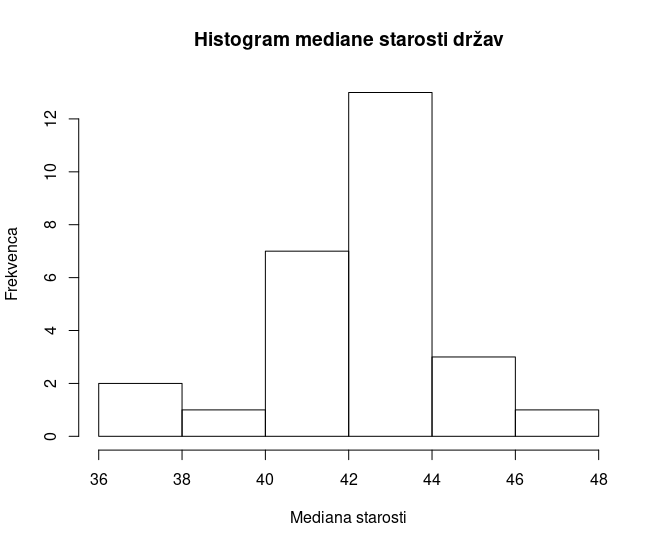
\includegraphics[scale=0.6]{histogram_mediane_starosti}\\
\end{center}
\begin{center}
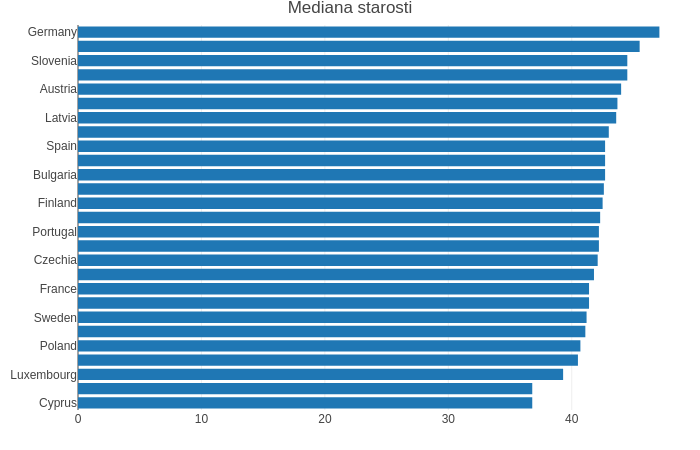
\includegraphics[scale=0.6]{barplot_mediane_starosti}\\
\end{center}
Iz histograma lahko sumimo, da je spremenljivka normalna ali simetrična. To lahko preverimo s Shapiro–Wilk testom. Naj bo ničelna hipoteza \(H_0\): spremenljivka je normalna in alternativna hipoteza \(H_1\): spremenljivka ni normalna. Izračunajmoga takole:
\[W = \frac{(\sum_{i = 1}^{n}a_i x_{(i)})^2}{\sum_{i = 1}^{n}(x_i - \overset{\_}{x})^2} = 0.94\]
kjer \(x_{(i)}\) je najmanjša vrednost v vzorcu, \(\overset{\_}{x}\) je povprečje median, \(a_i\) je i-ti element vektorja 0   
\[(a_1,...,a_n) = \frac{m^T V^{-1}}{C}\]
kjer \( C = \left\| V^{-1}m \right\|\) in vektor \(m = (m_1,...,m_n)^T\) je sestavljen iz pričakovanih vrednosti statističnih podatkov o vrstnem redu neodvisnih in identično razporejenih naključnih spremenljivk, vzorčenih iz standardne normalne porazdelitve. P vrednost za test je 
\[ p-value = 0.1218. \]
Izberemo 95\% interval zaupanja. \(\alpha\) je 0.05 (1 - 95\%). Če je vrednost p manjša od \(\alpha\), zavržemo \(H_0\). Ker je \(p > \alpha\) (0.1218 \(>\) 0.05), ne moremo zavreči ničelne hipoteze. Iz računa lahko slutimo, da spremenljivka ni normalno porazdeljena. Testiramo lahko, če je spremenljivka M simetrična. Računali bomo s Miao, Gel, and Gastwirth simetričnim testom. V R-ju je to ukaz symmetry.test(X, option = "MGG")\cite{lawstat}, kjer X je poljuben vektor. Naj bo ničelna hipoteza \(H_0\): Spremenljivka M je simetrična in alternativna hipoteza \(H_1\): spremenljivka M je asimterična. Za test spremenljivke S dobimo rezultate:
\[\text{Test statistike} = -0.42212 \text{ in p-value} =  0.684.\]
Tudi tukaj izberemo verjetnost 95\%, tako je \alpha = 0.05. Če je p vrednost \(< \alpha\), lahko zavrnemo hipotezo \(H_0\). Ker je p vrednost \(> \alpha\) (0.684 \(>\) 0.05) ne moremo zavrnit hipoteze \(H_0\). Zaradi velikega koeficienta p lahko smatramo, da je spremenljivka simetrična.


\subsubsection{Število dni do vrhunca prvega vala okuženih}
Spremenljivka S število dni do vrhunca prvega vala okuženih starosti je razlika v dnevih stolpcev DVO in DPO v bazi. Naprej lahko prikažemo spremenljivko z histogramom in barplotom. \\

\begin{center}
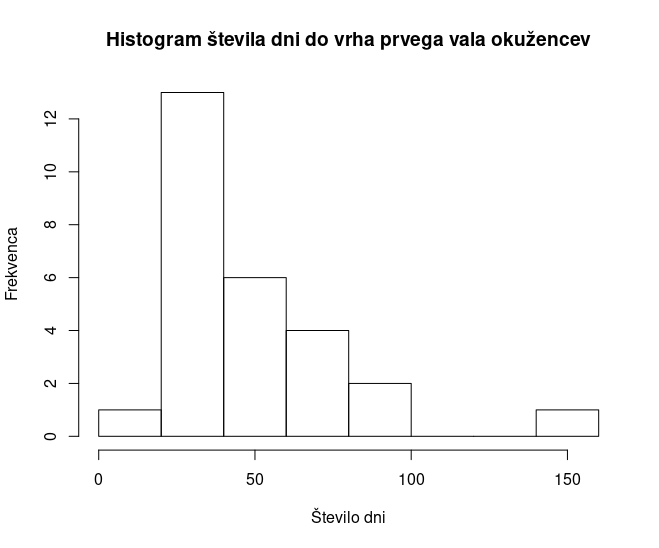
\includegraphics[scale=0.6]{histogram_st_dni_do_peaka_okuzencev}\\
\end{center}
\begin{center}
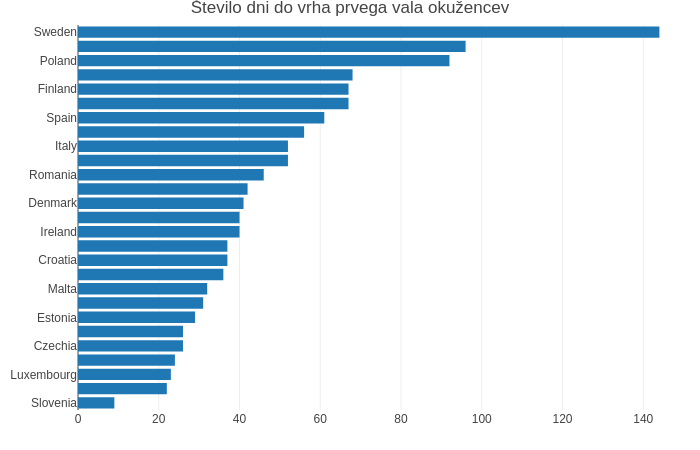
\includegraphics[scale=0.6]{barplot_st_dni_do_peaka_okuzencev}\\
\end{center}
Iz histograma ne moremo sumiti, da je spremenljivka normalna ali simetrična. To lahko preverimo s Shapiro–Wilk testom. Naj bo ničelna hipoteza \(H_0\): spremenljivka je normalna in alternativna hipoteza \(H_1\): spremenljivka ni normalna. Enak račun je narejen v paragrafu analize spremenljivke mediane straosti. Izračunajmoga takole:
\[W = \frac{(\sum_{i = 1}^{n}a_i x_{(i)})^2}{\sum_{i = 1}^{n}(x_i - \overset{\_}{x})^2} = 0.85.\]
 P vrednost za test je 
\[ p-value = 0.00126. \]
Izberemo 95\% interval zaupanja. \(\alpha\) je 0.05 (1 - 95\%). Če je vrednost p manjša od \(\alpha\), zavržemo \(H_0\). Ker je \(p < \alpha\) (0.00126 \(<\) 0.05), zavržemo ničelno hipotezo. Spremenljivka ni normalno porazdeljena, a to še ne pomeni, da ni simetrična. To preverimo s testom simetrije. Računali bomo s Miao, Gel, and Gastwirth simetričnim testom. V R-ju je to ukaz symmetry.test(X, option = "MGG")\cite{lawstat}, kjer X je poljuben vektor. Naj bo ničelna hipoteza \(H_0\): Spremenljivka S je simetrična in alternativna hipoteza \(H_1\): spremenljivka S je asimterična. Za test spremenljivke S dobimo rezultate:
\[\text{Test statistike} = 2.3151 \text{ in p-value} = 0.052.\]
Tudi tukaj izberemo verjetnost 95\%, tako je \alpha = 0.05. Če je p vrednost \(< \alpha\), lahko zavrnemo hipotezo \(H_0\). Ker je p vrednost \(> \alpha\) (0.052 \(>\) 0.05) ne moremo zavrnit hipoteze \(H_0\).

\subsubsection{Število dni do vrhunca prvega vala mrtvih}
Spremenljivka S število dni do vrhunca prvega vala mrtvih je razlika v dnevih stolpcev DVS in DPS v bazi. Naprej lahko prikažemo spremenljivko z histogramom in barplotom.\\

\begin{center}
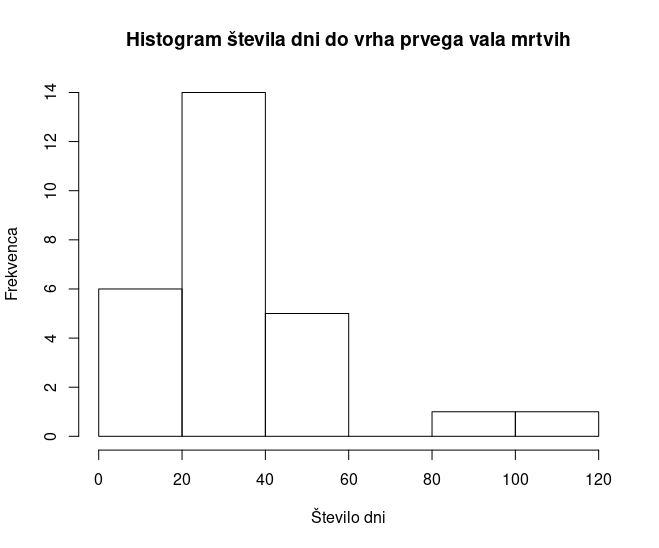
\includegraphics[scale=0.6]{histogram_st_dni_do_peaka_mrtvih}\\
\end{center}
\begin{center}
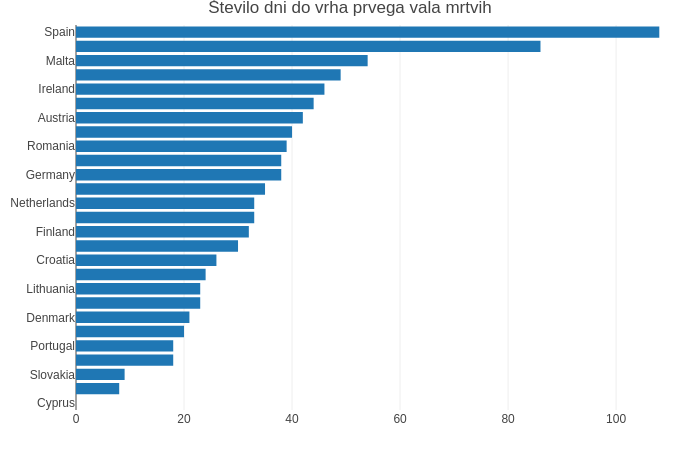
\includegraphics[scale=0.6]{barplot_st_dni_do_peaka_mrtvih}\\
\end{center}
Iz histograma ne moremo sumiti, da je spremenljivka normalna ali simetrična. To lahko preverimo s Shapiro–Wilk testom. Naj bo ničelna hipoteza \(H_0\): spremenljivka je normalna in alternativna hipoteza \(H_1\): spremenljivka ni normalna. Enak račun je narejen v paragrafu analize spremenljivke mediane straosti. Izračunajmoga takole:
\[W = \frac{(\sum_{i = 1}^{n}a_i x_{(i)})^2}{\sum_{i = 1}^{n}(x_i - \overset{\_}{x})^2} = 0.86235\]
 P vrednost za test je 
\[ p-value = 0.00204. \]
Izberemo 95\% interval zaupanja. \(\alpha\) je 0.05 (1 - 95\%). Če je vrednost p manjša od \(\alpha\), zavržemo \(H_0\). Ker je \(p < \alpha\) (0.00204 \(<\) 0.05), zavržemo ničelno hipotezo. Spremenljivka ni normalno porazdeljena, a to še ne pomeni, da ni simetrična. To preverimo s testom simetrije. Računali bomo s Miao, Gel, and Gastwirth simetričnim testom. V R-ju je to ukaz symmetry.test(X, option = "MGG")\cite{lawstat}, kjer X je poljuben vektor. Naj bo ničelna hipoteza \(H_0\): Spremenljivka S je simetrična in alternativna hipoteza \(H_1\): spremenljivka S je asimterična. Za test spremenljivke S dobimo rezultate:
\[\text{Test statistike} = 0.63107 \text{ in p-value} =  0.59.\]
Tudi tukaj izberemo verjetnost 95\%, tako je \alpha = 0.05. Če je p vrednost \(< \alpha\), lahko zavrnemo hipotezo \(H_0\). Ker je p vrednost \(> \alpha\) (0.59 \(>\) 0.05) ne moremo zavrnit hipoteze \(H_0\).

\subsubsection{Delež okuženih do vrhunca prvega vala okuženih}
Spremenljivka D delež okuženih do vrhunca prvega vala okuženih definiramo:
\[D = \frac{100 * \text{št. okuženih}}{\text{št. prebivalcev}}\]
kjer število okuženih je stolpec OV v bazi in število prebivalcev je stolpec PREB v bazi. Naprej lahko prikažemo spremenljivko D z histogramom in barplotom.\\
\begin{center}
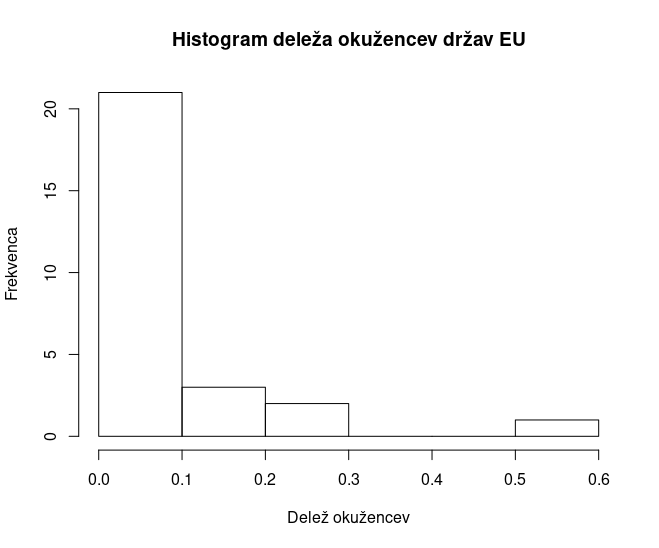
\includegraphics[scale=0.6]{histogram_delez_okuzenih}\\
\end{center}
\begin{center}
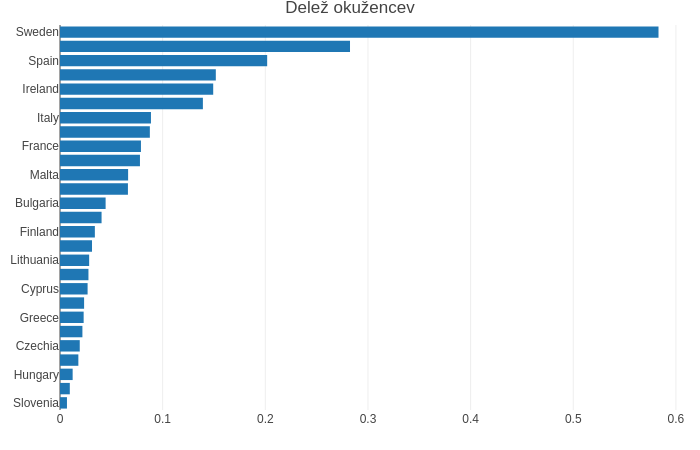
\includegraphics[scale=0.6]{barplot_delez_okuzenih}\\
\end{center}
Iz grafov je razvidno, da spremenljivka ni normalna in ni simetrična. To lahko potrdimo s Shapiro–Wilk testom. Naj bo ničelna hipoteza \(H_0\): spremenljivka je normalna in alternativna hipoteza \(H_1\): spremenljivka ni normalna. Enak račun je narejen v paragrafu analize spremenljivke mediane straosti. Izračunajmoga takole:
\[W = \frac{(\sum_{i = 1}^{n}a_i x_{(i)})^2}{\sum_{i = 1}^{n}(x_i - \overset{\_}{x})^2} = 0.62339\]
 P vrednost za test je 
\[ p-value = 3.925e-07. \]
Izberemo 95\% interval zaupanja. \(\alpha\) je 0.05 (1 - 95\%). Če je vrednost p manjša od \(\alpha\), zavržemo \(H_0\). Ker je \(p < \alpha\) (3.925e-07 \(<\) 0.05), zavržemo ničelno hipotezo. Spremenljivka ni normalno porazdeljena, a to še ne pomeni, da ni simetrična. To preverimo s testom simetrije. Računali bomo s Miao, Gel, and Gastwirth simetričnim testom. Naj bo ničelna hipoteza \(H_0\): Spremenljivka D je simetrična in alternativna hipoteza \(H_1\): spremenljivka D je asimterična. Za test spremenljivke S dobimo rezultate:
\[\text{Test statistike} = 3.9434 \text{ in p-value} =  0.002.\]
Tudi tukaj izberemo verjetnost 95\%, tako je \alpha = 0.05. Če je p vrednost \(< \alpha\), lahko zavrnemo hipotezo \(H_0\). Ker je p vrednost \(< \alpha\) (0.002 \(<\) 0.05) zavrnemo hipotezo \(H_0\). Spremenčjivka D ni normalno porazdeljena in je asimetrična. Delež okužencev je le vzorec, saj v ta delež niso šteti asimpotomatiki. Zaradi tega lahko izračunamo interval zaupanja za vsak delež okuženih. Računamo:
\[\Delta = t_{(1 + \beta) /2}(\infty) \times \sqrt{\frac{p(1 - p)}{n}}\]
kjer n je število prebivalcev države, p je delež okuženih, \(\Delta\) je razmik intervala, \(t_{p}(r)\) je vrednost studentove t-porazdelitve s r stopnjami svobode in p procent zaupanja. Izbrana \(\beta\) je 0.95, kar pomeni, da je \(\alpha = \) 0.05. Izračunan interval je prikazan v spodnji tabeli. \\
\scalebox{1.0}{
\csvautotabular{dbIntervalZaupanjaDelezOkuzenih.csv}
}

\subsubsection{Delež mrtvih do vrhunca prvega vala okuženih}
Spremenljivka D delež okuženih do vrhunca prvega vala okuženih definiramo:
\[D = \frac{100 * \text{št. mrtvih}}{\text{št. okuženih}}\]
kjer število okuženih je stolpec MV v bazi in število prebivalcev je stolpec OV v bazi. Naprej lahko prikažemo spremenljivko D z histogramom in barplotom.\\
\begin{center}
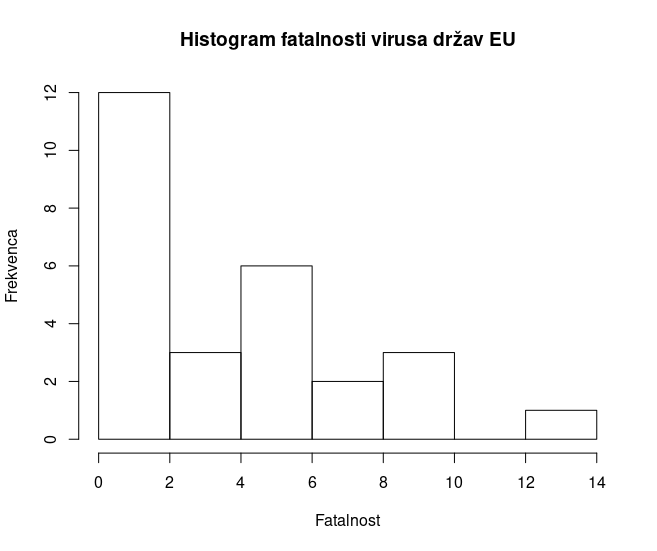
\includegraphics[scale=0.6]{histogram_fatalnost}\\
\end{center}
\begin{center}
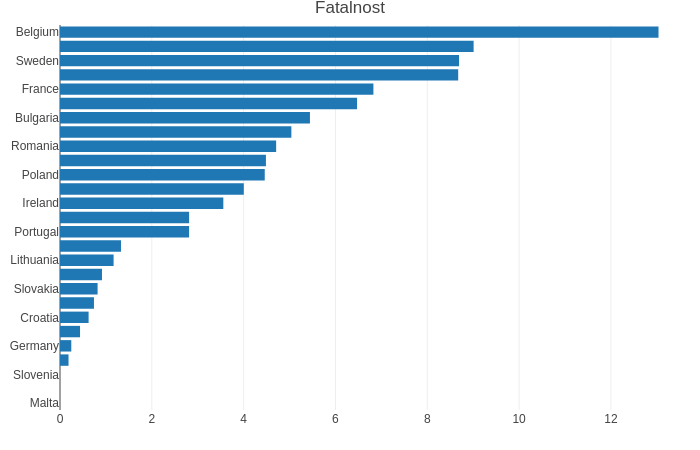
\includegraphics[scale=0.6]{barplot_fatalnost}\\
\end{center}
Iz grafov je razvidno, da spremenljivka ni normalna in ni simetrična. To lahko potrdimo s Shapiro–Wilk testom. Naj bo ničelna hipoteza \(H_0\): spremenljivka je normalna in alternativna hipoteza \(H_1\): spremenljivka ni normalna. Enak račun je narejen v paragrafu analize spremenljivke mediane straosti. Izračunajmoga takole:
\[W = \frac{(\sum_{i = 1}^{n}a_i x_{(i)})^2}{\sum_{i = 1}^{n}(x_i - \overset{\_}{x})^2} = 0.8851\]
 P vrednost za test je 
\[ p-value = 0.0062. \]
Izberemo 95\% interval zaupanja. \(\alpha\) je 0.05 (1 - 95\%). Če je vrednost p manjša od \(\alpha\), zavržemo \(H_0\). Ker je \(p < \alpha\) (0.0062 \(<\) 0.05), zavržemo ničelno hipotezo. Spremenljivka ni normalno porazdeljena, a to še ne pomeni, da ni simetrična. To preverimo s testom simetrije. Računali bomo s Miao, Gel, and Gastwirth simetričnim testom. Naj bo ničelna hipoteza \(H_0\): Spremenljivka D je simetrična in alternativna hipoteza \(H_1\): spremenljivka D je asimterična. Za test spremenljivke S dobimo rezultate:
\[\text{Test statistike} = 1.5009 \text{ in p-value} =  0.26.\]
Tudi tukaj izberemo verjetnost 95\%, tako je \alpha = 0.05. Če je p vrednost \(< \alpha\), lahko zavrnemo hipotezo \(H_0\). Ker je p vrednost \(> \alpha\) (0.26 \(>\) 0.05) ne moremo zavrniti hipotezo \(H_0\). Spremenčjivka D ni normalno porazdeljena in smatramo da je asimetrična, ker je p vrednost zadnejga testa zelo majhen. Kot v prejšnji analizu, delež okužencev je le vzorec, saj v ta delež niso šteti asimpotomatiki. Zaradi tega lahko izračunamo interval zaupanja za vsak delež okuženih. Računamo:
\[\Delta = t_{(1 + \beta) /2}(\infty) \times \sqrt{\frac{p(1 - p)}{n}}\]
kjer n je število prebivalcev države, p je delež okuženih, \(\Delta\) je razmik intervala, \(t_{p}(r)\) je vrednost studentove t-porazdelitve s r stopnjami svobode in p procent zaupanja. Izbrana \(\beta\) je 0.95, kar pomeni, da je \(\alpha = \) 0.05. Izračunan interval je prikazan v spodnji tabeli. \\
\scalebox{1.0}{
\csvautotabular{dbIntervalZaupanjaFatalnost.csv}
}

\subsubsection{Delež testov do vrhunca prvega vala okuženih}
Spremenljivka T delež testov do vrhunca prvega vala okuženih definiramo:
\[T = \frac{100 * \text{št. opravljenih testov}}{\text{št. prebivalcev}}\]
kjer število opravljenih je stolpec OTO v bazi in število prebivalcev je stolpec PREB v bazi. Naprej lahko prikažemo spremenljivko T s histogramom in barplotom.\\
\begin{center}
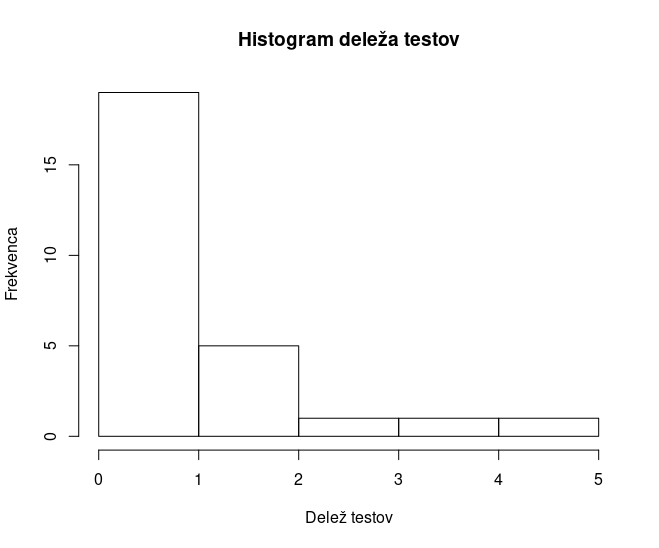
\includegraphics[scale=0.6]{histogram_delez_testov}\\
\end{center}
\begin{center}
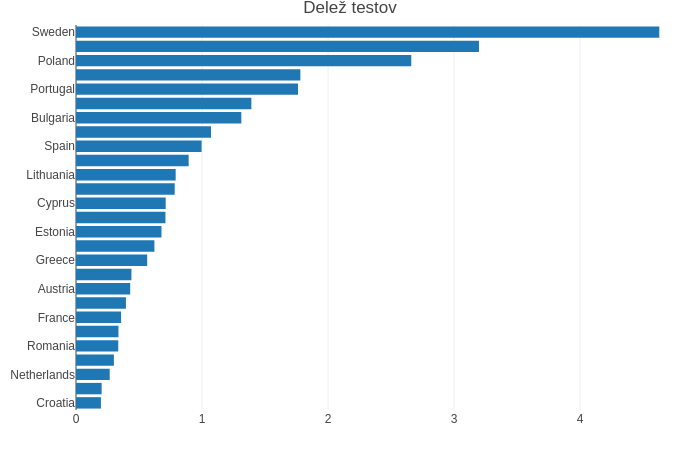
\includegraphics[scale=0.6]{barplot_delez_testov}\\
\end{center}
Iz grafov je razvidno, da spremenljivka ni normalna in ni simetrična. To lahko potrdimo s Shapiro–Wilk testom. Naj bo ničelna hipoteza \(H_0\): spremenljivka je normalna in alternativna hipoteza \(H_1\): spremenljivka ni normalna. Enak račun je narejen v paragrafu analize spremenljivke mediane straosti. Izračunajmoga takole:
\[W = \frac{(\sum_{i = 1}^{n}a_i x_{(i)})^2}{\sum_{i = 1}^{n}(x_i - \overset{\_}{x})^2} = 0.73562\]
 P vrednost za test je 
\[ p-value = 1.264e-05. \]
Izberemo 95\% interval zaupanja. \(\alpha\) je 0.05 (1 - 95\%). Če je vrednost p manjša od \(\alpha\), zavržemo \(H_0\). Ker je \(p < \alpha\) (1.264e-05 \(<\) 0.05), zavržemo ničelno hipotezo. Spremenljivka ni normalno porazdeljena, a to še ne pomeni, da ni simetrična. To preverimo s testom simetrije. Računali bomo s Miao, Gel, and Gastwirth simetričnim testom. Naj bo ničelna hipoteza \(H_0\): Spremenljivka T je simetrična in alternativna hipoteza \(H_1\): spremenljivka T je asimterična. Za test spremenljivke S dobimo rezultate:
\[\text{Test statistike} = 2.8186 \text{ in p-value} =  0.018.\]
Tudi tukaj izberemo verjetnost 95\%, tako je \alpha = 0.05. Če je p vrednost \(< \alpha\), lahko zavrnemo hipotezo \(H_0\). Ker je p vrednost \(< \alpha\) (0.018 \(<\) 0.05) zavrnemo ničelno hipotezo \(H_0\). Spremenčjivka T ni normalno porazdeljena in je asimetrična.

\subsection{Korelacijska analiza}
Korelacijsko analizo bom razdelil na tri dele in sicer:
\begin{enumerate}
\item{Mediana starosti}
\item{Delež testov starosti}
\item{Število dni do vrha prvega vala okuženih}
\end{enumerate}

\subsubsection{Mediana starosti}
Zanima me kako je mediana starosti vplivala na druge spremenljivke in sicer na število dni do vrhunca prvega vala okuženih, število dni do vrhunca prvega vala mrtvih, delež okuženih do vrhunca prvega vala okuženih, delež mrtvih do vrhunca prvega vala okuženih.

\paragraph{Vpliv mediane starosti na število dni do vrhunca prvega vala okuženih}
Sprašujemo se kakšna je korelacija med spremenljivko M mediana starosti (stolpec MED v bazi) in spremenljivko Š številom dni do vrhunca prvega vala okuženih. Podatke navedenoh spremenljivk lahkjo prikažemo z razsvenim grafom.
\\
\begin{center}
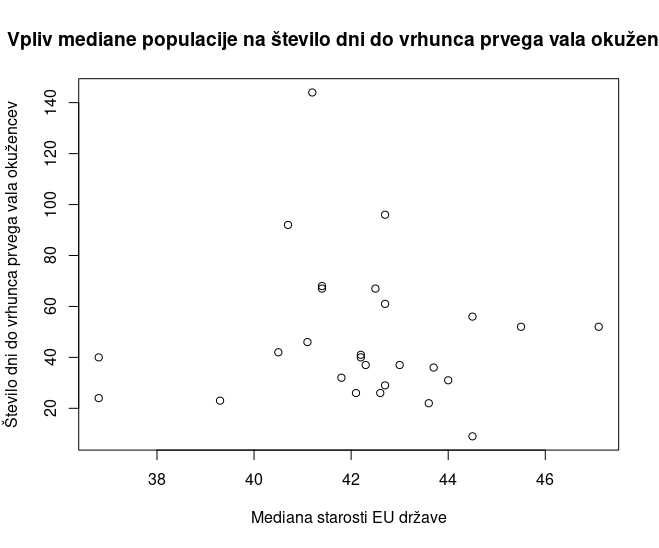
\includegraphics[scale=0.6]{vpliv_med_populacije_na_st_dni_do_peaka_okuezenih}\\
\end{center}
Koeficient korelacije lahko izračunamo s Pearsonovim koeficientom korelacije:

\begin{center}
\[\text{r} = \frac{Cov(M,Š)}{\sigma_{M} \sigma_{Š}} = -0.0258\]
\end{center} 
kjer je \(\sigma_{M}\) standardni odklon spremenljivke M in \(\sigma_{Š}\) standardni odklon spremenljivke Š. Koeficient ni dovolj velik, da bi lahko smatrali, da obstaja močna povezanost med spremenljivkima. Pravzaprav ker je tako blizu ničle lahko smatramo, da sta si spremenljivki M in Š neodvisni, a to ni še gotovo. Menda sta si spremenljivke nelinearno povezane. To lahko preverimo s Spearmanovim koeficientom korelacije. Izračunajmoga takole: 

\begin{center}
\[\rho = 1 - \frac{6\sum_{i}{}d_i^2}{N(N^2 - 1)} = -0.0888\]
\end{center} 

kjer je \( d_i \) razlika med rangoma za i-to enoto in N pa število vseh enot (parov rangov). Tudi Spearmanov koeficient je zelo majhen, negativen in blizu ničli. Ponovno slutimo, da sta si spremenljivki M in Š neodvisni.
Ker je število okuženecv le vzorec, ker niso šteti asimptomatiki, lahko izračunamo interval zaupanja za korelacijski koeficient. V R-ju lahko izračunamo 95\% interval zaupanja z ukazom cor.test(M,Š, method = "pearson").
\[[r - \Delta, r + \Delta] = [-0.4019, 0.3577]\]
Da bi bile spremenljivke M in Š v korelaciji, bi moral biti koeficient korelacije večji od 0.7 ali manjši od -0.7. Nobena vrednost v zgornejm intervalu, ne zadošča pogoju zaradi tega lahko smatramo, da sta si spremenljivki M in Š neodvisni.

\paragraph{Vpliv mediane starosti na število dni do vrhunca prvega vala mrtvih}
Sprašujemo se kakšna je korelacija med spremenljivko M mediana starosti (stolpec MED v bazi) in spremenljivko Š številom dni do vrhunca prvega vala mrtvih. Podatke navedenih spremenljivk lahko prikažemo z razsvenim grafom.
\\
\begin{center}
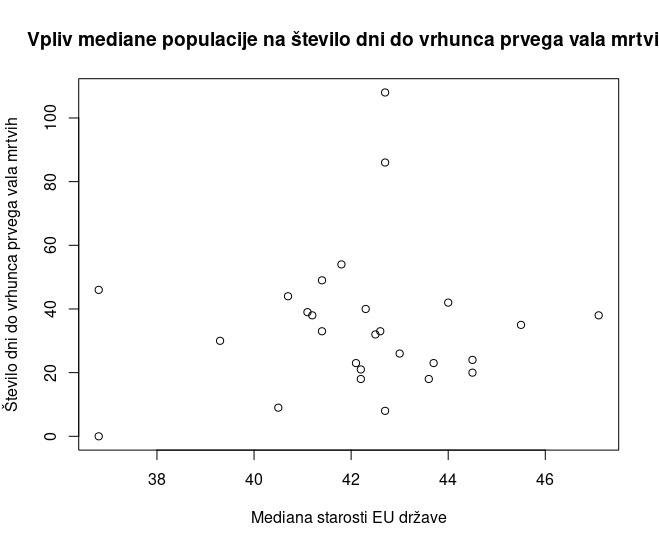
\includegraphics[scale=0.6]{vpliv_med_pop_na_st_dni_do_peaka_mrtvih}\\
\end{center}
Koeficient korelacije lahko izračunamo s Pearsonovim koeficientom korelacije:

\begin{center}
\[\text{r} = \frac{Cov(M,Š)}{\sigma_{M} \sigma_{Š}} = 0.0902\]
\end{center} 
kjer je \(\sigma_{M}\) standardni odklon spremenljivke M in \(\sigma_{Š}\) standardni odklon spremenljivke Š. Koeficient ni dovolj velik, da bi lahko smatrali, da obstaja močna povezanost med spremenljivkima. Pravzaprav ker je tako blizu ničle lahko smatramo, da sta si spremenljivki M in Š neodvisni, a to ni še gotovo. Menda sta si spremenljivke nelinearno povezane. To lahko preverimo s Spearmanovim koeficientom korelacije. Izračunajmoga takole: 

\begin{center}
\[\rho = 1 - \frac{6\sum_{i}{}d_i^2}{N(N^2 - 1)} = -0.052\]
\end{center} 

kjer je \( d_i \) razlika med rangoma za i-to enoto in N pa število vseh enot (parov rangov). Tudi Spearmanov koeficient je zelo majhen, negativen in blizu ničli. Ponovno slutimo, da sta si spremenljivki M in Š neodvisni.
Ker je število okuženecv le vzorec, ker niso šteti asimptomatiki, lahko izračunamo interval zaupanja za korelacijski koeficient. V R-ju lahko izračunamo 95\% interval zaupanja z ukazom cor.test(M,Š, method = "pearson").
\[[r - \Delta, r + \Delta] = [-0.3001382, 0.4545977]\]
Da bi bile spremenljivke M in Š v korelaciji, bi moral biti koeficient korelacije večji od 0.7 ali manjši od -0.7. Nobena vrednost v zgornejm intervalu, ne zadošča pogoju zaradi tega lahko smatramo, da sta si spremenljivki M in Š neodvisni.

\paragraph{Vpliv mediane starosti na delež okuženih do vrhunca prvega vala okuženih}
Sprašujemo se kakšna je korelacija med spremenljivko M mediana starosti (stolpec MED v bazi) in spremenljivko D delež okuženih do vrhunca prvega vala okuženih. Najprej definirajmo spremenljivko D:
\[D = \frac{100 * \text{št. okuženih}}{\text{št. prebivalcev}}\]
kjer število okuženih je stolpec OV v bazi in število prebivalcev je stolpec PREB v bazi. Podatke navedenih spremenljivk lahko prikažemo z razsvenim grafom.
\\
\begin{center}
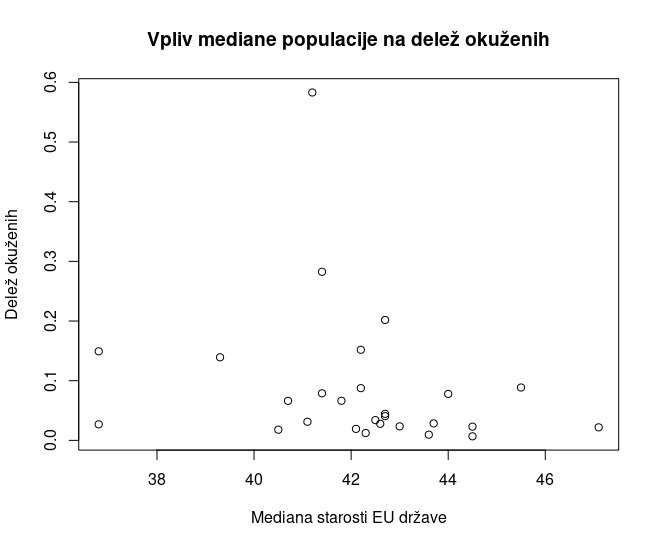
\includegraphics[scale=0.6]{vpliv_med_pop_na_delez_okuzencev}\\
\end{center}
Koeficient korelacije lahko izračunamo s Pearsonovim koeficientom korelacije:

\begin{center}
\[\text{r} = \frac{Cov(M,D)}{\sigma_{M} \sigma_{D}} = -0.2203\]
\end{center} 
kjer je \(\sigma_{M}\) standardni odklon spremenljivke M in \(\sigma_{D}\) standardni odklon spremenljivke D. Koeficient ni dovolj velik, da bi lahko smatrali, da obstaja močna povezanost med spremenljivkima. Pravzaprav ker je tako blizu ničle lahko smatramo, da sta si spremenljivki M in Š neodvisni, a to ni še gotovo. Menda sta si spremenljivke nelinearno povezane. To lahko preverimo s Spearmanovim koeficientom korelacije. Izračunajmoga takole: 

\begin{center}
\[\rho = 1 - \frac{6\sum_{i}{}d_i^2}{N(N^2 - 1)} = -0.3255\]
\end{center} 

kjer je \( d_i \) razlika med rangoma za i-to enoto in N pa število vseh enot (parov rangov). Tudi Spearmanov koeficient je zelo majhen, negativen in blizu ničli. Ponovno slutimo, da sta si spremenljivki M in D neodvisni.
Ker je število okuženecv le vzorec, ker niso šteti asimptomatiki, lahko izračunamo interval zaupanja za korelacijski koeficient. V R-ju lahko izračunamo 95\% interval zaupanja z ukazom cor.test(M,Š, method = "pearson").
\[[r - \Delta, r + \Delta] = [-0.5539, 0.1743]\]
Da bi bile spremenljivke M in D v korelaciji, bi moral biti koeficient korelacije večji od 0.7 ali manjši od -0.7. Nobena vrednost v zgornejm intervalu, ne zadošča pogoju zaradi tega lahko smatramo, da sta si spremenljivki M in D neodvisni.

\paragraph{Vpliv mediane starosti na delež mrtvih do vrhunca prvega vala okuženih}
Sprašujemo se kakšna je korelacija med spremenljivko M mediana starosti (stolpec MED v bazi) in spremenljivko D delež mrtvih do vrhunca prvega vala okuženih. Najprej definirajmo spremenljivko D:
\[D = \frac{100 * \text{št. mrtvih}}{\text{št. okuženih}}\]
kjer število okuženih je stolpec MV v bazi in število prebivalcev je stolpec OV v bazi. Podatke navedenih spremenljivk lahko prikažemo z razsvenim grafom.
\\
\begin{center}
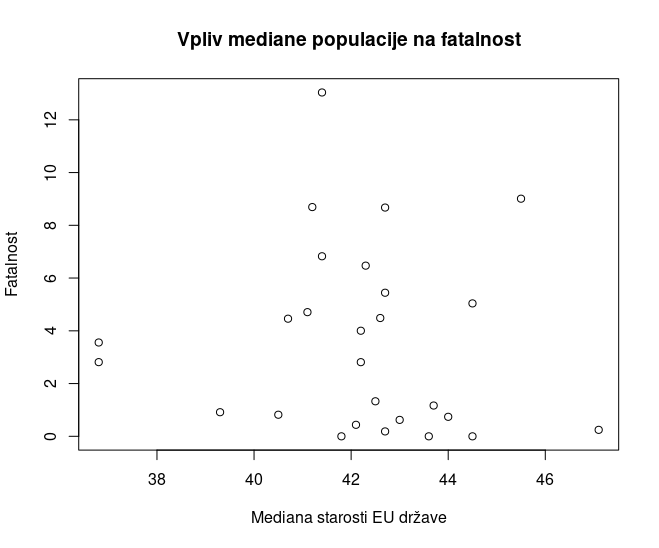
\includegraphics[scale=0.6]{vpliv_med_pop_na_fatalnost}\\
\end{center}
Koeficient korelacije lahko izračunamo s Pearsonovim koeficientom korelacije:

\begin{center}
\[\text{r} = \frac{Cov(M,D)}{\sigma_{M} \sigma_{D}} = -0.0845\]
\end{center} 
kjer je \(\sigma_{M}\) standardni odklon spremenljivke M in \(\sigma_{D}\) standardni odklon spremenljivke D. Koeficient ni dovolj velik, da bi lahko smatrali, da obstaja močna povezanost med spremenljivkima. Pravzaprav ker je tako blizu ničle lahko smatramo, da sta si spremenljivki M in D neodvisni, a to ni še gotovo. Menda sta si spremenljivke nelinearno povezane. To lahko preverimo s Spearmanovim koeficientom korelacije. Izračunajmoga takole: 

\begin{center}
\[\rho = 1 - \frac{6\sum_{i}{}d_i^2}{N(N^2 - 1)} = -0.1951\]
\end{center} 

kjer je \( d_i \) razlika med rangoma za i-to enoto in N pa število vseh enot (parov rangov). Tudi Spearmanov koeficient je zelo majhen, negativen in blizu ničli. Ponovno slutimo, da sta si spremenljivki M in D neodvisni.
Ker je število okuženecv le vzorec, ker niso šteti asimptomatiki, lahko izračunamo interval zaupanja za korelacijski koeficient. V R-ju lahko izračunamo 95\% interval zaupanja z ukazom cor.test(M,Š, method = "pearson").
\[[r - \Delta, r + \Delta] = [-0.45, 0.3053]\]
Da bi bile spremenljivke M in D v korelaciji, bi moral biti koeficient korelacije večji od 0.7 ali manjši od -0.7. Nobena vrednost v zgornejm intervalu, ne zadošča pogoju zaradi tega lahko smatramo, da sta si spremenljivki M in D neodvisni.

\subsubsection{Delež testov}

Zanima me kako je delež testov vpliva na druge spremenljivke in sicer na delež okuženih do vrhunca prvega vala okuženi in na delež mrtvih do vrhunca prvega vala okuženih. Definirajmo spremenljivko T delež testov:
\[T = \frac{100 * \text{št. opravljenih testov}}{\text{št. prebivalcev}}\]
kjer število opravljenih je stolpec OTO v bazi in število prebivalcev je stolpec PREB v bazi.

\paragraph{Vpliv delež testov na delež okuženih do vrhunca prvega vala okuženih}
Sprašujemo se kakšna je korelacija med spremenljivko T in spremenljivko D delež mrtvih do vrhunca prvega vala okuženih. Najprej definirajmo spremenljivko D:
\[D = \frac{100 * \text{št. okuženih}}{\text{št. prebivalcev}}\]
kjer število okuženih je stolpec OV v bazi in število prebivalcev je stolpec PREB v bazi. Podatke navedenih spremenljivk lahko prikažemo z razsvenim grafom.
\\
\begin{center}
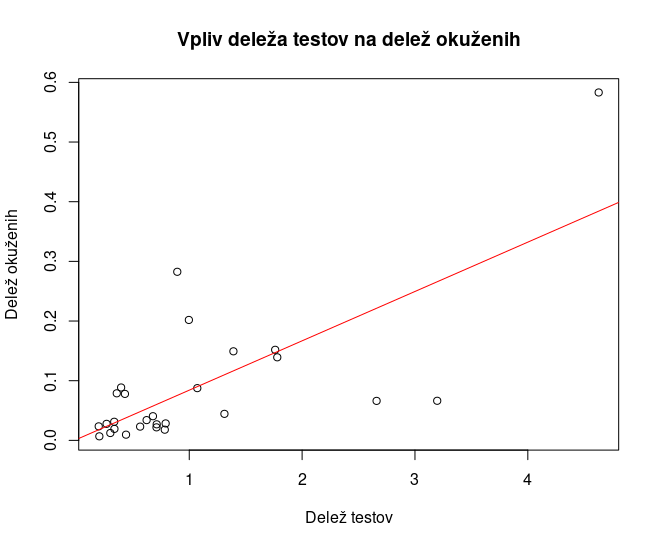
\includegraphics[scale=0.6]{vpliv_deleza_testov_na_delez_okuzenih}\\
\end{center}
Iz grafa lahko zaznamo nek trend med spremenljivkama. Koeficient korelacije lahko izračunamo s Pearsonovim koeficientom korelacije:

\begin{center}
\[\text{r} = \frac{Cov(M,D)}{\sigma_{M} \sigma_{D}} = 0.7131\]
\end{center} 
kjer je \(\sigma_{M}\) standardni odklon spremenljivke M in \(\sigma_{D}\) standardni odklon spremenljivke D. Koeficient je dovolj velik, da bi lahko smatrali, da obstaja močna povezanost med spremenljivkima. lahko trdimo, da spremenljivki sta si odvisni.
Ker je število okuženecv le vzorec, ker niso šteti asimptomatiki, lahko izračunamo interval zaupanja za korelacijski koeficient. V R-ju lahko izračunamo 95\% interval zaupanja z ukazom cor.test(M,Š, method = "pearson").
\[[r - \Delta, r + \Delta] = [0.4568, 0.86]\]
Da bi bile spremenljivke M in D v korelaciji, bi moral biti koeficient korelacije večji od 0.7 ali manjši od -0.7.

\paragraph{Vpliv delež testov na delež mrtvih do vrhunca prvega vala okuženih}
Sprašujemo se kakšna je korelacija med spremenljivko M mediana starosti (stolpec MED v bazi) in spremenljivko D delež mrtvih do vrhunca prvega vala okuženih. Najprej definirajmo spremenljivko D:
\[D = \frac{100 * \text{št. mrtvih}}{\text{št. okuženih}}\]
kjer število mrtvih je stolpec MV v bazi in število okuženih je stolpec OV v bazi. Podatke navedenih spremenljivk lahko prikažemo z razsvenim grafom.
\\
\begin{center}
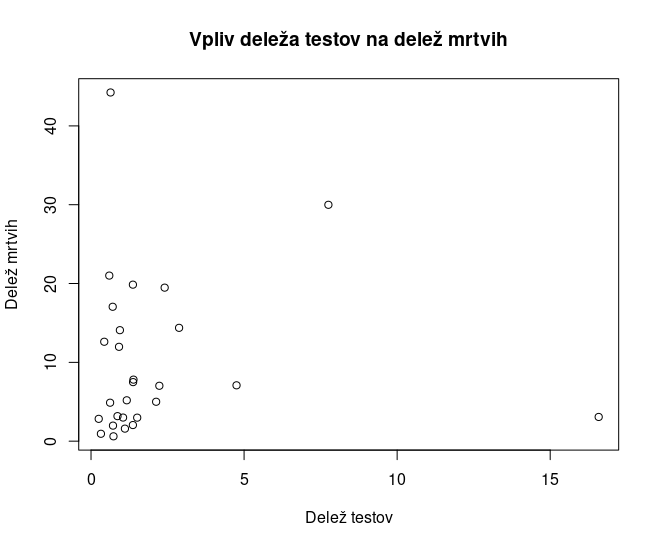
\includegraphics[scale=0.6]{vpliv_delez_testov_na_delez_mrtvih}\\
\end{center}
Koeficient korelacije lahko izračunamo s Pearsonovim koeficientom korelacije:

\begin{center}
\[\text{r} = \frac{Cov(T,D)}{\sigma_{T} \sigma_{D}} = 0.1596\]
\end{center} 
kjer je \(\sigma_{T}\) standardni odklon spremenljivke T in \(\sigma_{D}\) standardni odklon spremenljivke D. Koeficient ni dovolj velik, da bi lahko smatrali, da obstaja močna povezanost med spremenljivkima. Pravzaprav ker je tako blizu ničle lahko smatramo, da sta si spremenljivki T in D neodvisni, a to ni še gotovo. Menda sta si spremenljivke nelinearno povezane. To lahko preverimo s Spearmanovim koeficientom korelacije. Izračunajmoga takole: 

\begin{center}
\[\rho = 1 - \frac{6\sum_{i}{}d_i^2}{N(N^2 - 1)} = 0.1246\]
\end{center} 

kjer je \( d_i \) razlika med rangoma za i-to enoto in N pa število vseh enot (parov rangov). Tudi Spearmanov koeficient je zelo majhen, negativen in blizu ničli. Ponovno slutimo, da sta si spremenljivki T in D neodvisni.
Ker je število okuženecv le vzorec, ker niso šteti asimptomatiki, lahko izračunamo interval zaupanja za korelacijski koeficient. V R-ju lahko izračunamo 95\% interval zaupanja z ukazom cor.test(T,D, method = "pearson").
\[[r - \Delta, r + \Delta] = [-0.45, 0.3053]\]
Da bi bile spremenljivke T in D v korelaciji, bi moral biti koeficient korelacije večji od 0.7 ali manjši od -0.7. Nobena vrednost v zgornejm intervalu, ne zadošča pogoju zaradi tega lahko smatramo, da sta si spremenljivki T in D neodvisni.

\subsubsection{Število dni do vrha prvega vala okuženih}

Zanima me kako je število dni do vrha prvega vala okuženih vpliva na druge spremenljivke in sicer na delež okuženih do vrhunca prvega vala okuženi in na delež mrtvih do vrhunca prvega vala okuženih. Spremenljivka Š število dni do vrhunca prvega vala okuženih starosti je razlika v dnevih
stolpcev DVO in DPO v bazi.

\paragraph{Vpliv število dni do vrha prvega vala okuženih na delež okuženih do vrhunca prvega vala okuženih}
Sprašujemo se kakšna je korelacija med spremenljivko Š in spremenljivko D delež mrtvih do vrhunca prvega vala okuženih. Najprej definirajmo spremenljivko D:
\[D = \frac{100 * \text{št. okuženih}}{\text{št. prebivalcev}}\]
kjer število okuženih je stolpec OV v bazi in število prebivalcev je stolpec PREB v bazi. Podatke navedenih spremenljivk lahko prikažemo z razsvenim grafom.
\\
\begin{center}
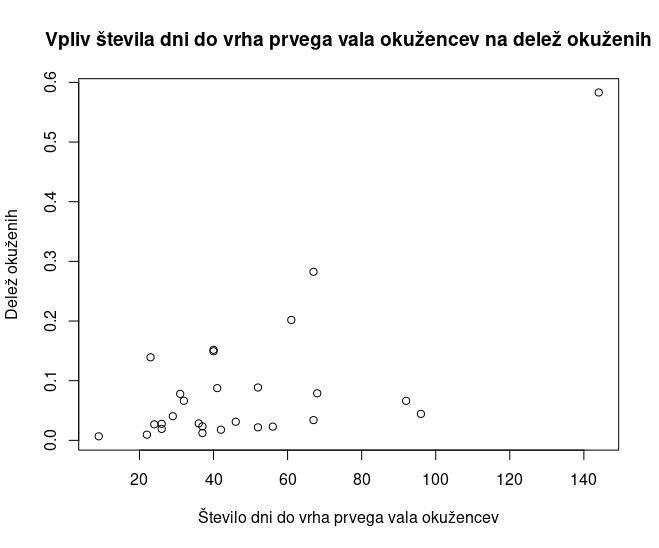
\includegraphics[scale=0.6]{vpliv_stevila_dni_do_peaka_okuzencev_na_delez_okuzenih}\\
\end{center}
Iz grafa lahko zaznamo nek trend med spremenljivkama. Koeficient korelacije lahko izračunamo s Pearsonovim koeficientom korelacije:

\begin{center}
\[\text{r} = \frac{Cov(Š,D)}{\sigma_{Š} \sigma_{D}} = 0.67554\]
\end{center} 
kjer je \(\sigma_{Š}\) standardni odklon spremenljivke Š in \(\sigma_{D}\) standardni odklon spremenljivke D. Koeficient ni dovolj velik, ker je manjši od 0.7, da bi lahko smatrali, da obstaja močna povezanost med spremenljivkima. Ne moremo trditi, da spremenljivki sta si odvisni. Menda sta si spremenljivke nelinearno povezane. To lahko preverimo s Spearmanovim koeficientom korelacije. Izračunajmoga takole: 

\begin{center}
\[\rho = 1 - \frac{6\sum_{i}{}d_i^2}{N(N^2 - 1)} = 0.4573\]
\end{center}

kjer je \( d_i \) razlika med rangoma za i-to enoto in N pa število vseh enot (parov rangov). Tudi Spearmanov koeficient je manjši od 0.7. Ponovno slutimo, da sta si spremenljivki Š in D neodvisni.
Ker je število okuženecv le vzorec, ker niso šteti asimptomatiki, lahko izračunamo interval zaupanja za korelacijski koeficient. V R-ju lahko izračunamo 95\% interval zaupanja z ukazom cor.test(M,Š, method = "pearson").
\[[r - \Delta, r + \Delta] = [0.3976, 0.8399]\]
Da bi bile spremenljivke Š in D v korelaciji, bi moral biti koeficient korelacije večji od 0.7 ali manjši od -0.7. Del zgornjega intervala je večji od 0.7. Če bi korelacijski koeficient populacije večji od 0.7 bi lahko z gotovstjo trdili, da obstaja močna povezanost med spremenljivkima Š in D.

\paragraph{Vpliv delež testov na delež mrtvih do vrhunca prvega vala okuženih}
Sprašujemo se kakšna je korelacija med spremenljivko T in spremenljivko D delež mrtvih do vrhunca prvega vala okuženih. Najprej definirajmo spremenljivko D:
\[D = \frac{100 * \text{št. mrtvih}}{\text{št. okuženih}}\]
kjer število mrtvih je stolpec MV v bazi in število okuženih je stolpec OV v bazi. Podatke navedenih spremenljivk lahko prikažemo z razsvenim grafom.
\\
\begin{center}
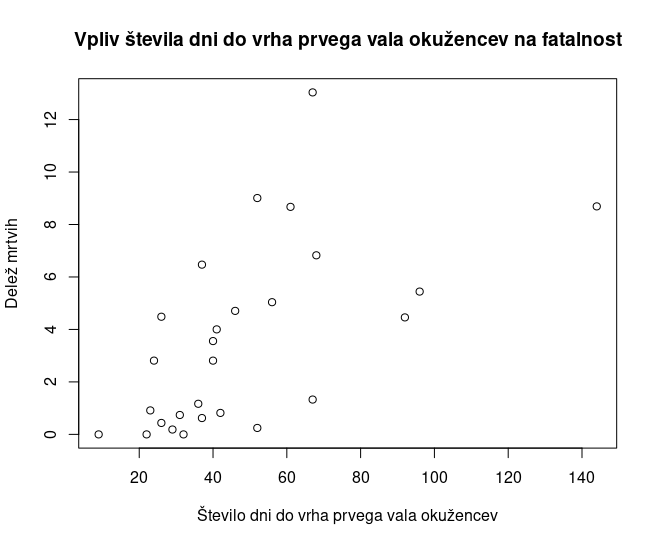
\includegraphics[scale=0.6]{vpliv_stevila_dni_do_peaka_okuzencev_na_fatalnost}\\
\end{center}
Koeficient korelacije lahko izračunamo s Pearsonovim koeficientom korelacije:

\begin{center}
\[\text{r} = \frac{Cov(Š,D)}{\sigma_{Š} \sigma_{D}} = 0.5856\]
\end{center} 
kjer je \(\sigma_{Š}\) standardni odklon spremenljivke Š in \(\sigma_{D}\) standardni odklon spremenljivke D. Koeficient ni dovolj velik, da bi lahko smatrali, da obstaja močna povezanost med spremenljivkima. Pravzaprav ker je tako blizu ničle lahko smatramo, da sta si spremenljivki T in D neodvisni, a to ni še gotovo. Menda sta si spremenljivke nelinearno povezane. To lahko preverimo s Spearmanovim koeficientom korelacije. Izračunajmoga takole: 

\begin{center}
\[\rho = 1 - \frac{6\sum_{i}{}d_i^2}{N(N^2 - 1)} = 0.6868\]
\end{center} 

kjer je \( d_i \) razlika med rangoma za i-to enoto in N pa število vseh enot (parov rangov). Tudi Spearmanov koeficient je zelo majhen, negativen in blizu ničli. Ponovno slutimo, da sta si spremenljivki T in D neodvisni.
Ker je število okuženecv le vzorec, ker niso šteti asimptomatiki, lahko izračunamo interval zaupanja za korelacijski koeficient. V R-ju lahko izračunamo 95\% interval zaupanja z ukazom cor.test(T,D, method = "pearson").
\[[r - \Delta, r + \Delta] = [0.2644, 0.7898]\]
Da bi bile spremenljivke Š in D v korelaciji, bi moral biti koeficient korelacije večji od 0.7 ali manjši od -0.7. Le majhen del zgornjega intervala zadošča pogoju zaradi tega lahko smatramo, da sta si spremenljivki Š in D linearno nekorelirani.

\section{Zaključki}
Iz analize spremenljivk lahko sklepamo, da je spremenljivka mediane starosti normalno porazdeljena, kar je smiselno za države v istem območju in z podobnimi življenskimi dobami. Spremenljivke: število dni do vrhunca prvega vala okuženih, števila dni do vrhunca prvega vala mrtvih, delež okuženih, delež mrtvih in delež testov niso normalno porazdeljene. Sklepamo lahko, da na te spremenljivke vpliva čas, ki je potrebovala posamezna država za regulacije (maske, rokavice in socialno distanciranje), saj vsaka država je ukrepala poljubno. \\
Iz korelacijske analiza lahko smatramo, da spremenljivka mediane starosti ni ne korelirana linearno ali nelinerano na število dni do vrhunca prvega vala okuženih, število dni do vrhunca prvega vala mrtvih, delež okuženih do vrhunca prvega vala okuženih, delež mrtvih do vrhunca prvega vala okuženih. Naj bo 0.7 meja za povezanost med dvemi spremenljivkam. Če je njihov korelacijski koeficient večji od 0.7 lahko smatramo da sta si pozitivno močno povezani. Če je njihov korelacijski koeficient manjši od -0.7 lahko smatramo da sta si negativno močno povezani.Tudi intervali zaupnja vseh štirih korelacij ne vsebujejo nobene vrednosti večje od 0.7 ali manjše od -0.7 zaradi tega se iz računov sluti, da spremenljivka mediana starosti ne vpliva na ostale izbrane spremenljivke. \\
Korelacijska analiza deleža testov in drugih izbranih spremenljivk je privedla do zanimivih rezultatov. Izkaže se, da je spremenljivka deleža testov linearno povezana z deležom okuženih, saj če država opravi več testov lahko zazna več okužencev. Enako se ne izkaže za fatalnost virusa. Na fatalnost vplivajo tudi drugi faktorji, kot so zmogljivost bolnišnic in če je bolnik imel še druge bolezni. \\
Korelacijska analiza število dni do vrha prvega vala okuženih in drugih izbranih spremenljivk je tudi privedla do zanimivih rezultatov. Stevilo dni do vrha prvega vala okuženih in delež okuženih sta si skoraj linearno povezani. Lahko zaklučimo, da je smiselno, da obstaja neka povezanost med spremenljivkima, saj v večjem številu dni se lahko zazna več okuženih ljudi. Podobno velja za spremenljivki število dni do vrha prvega vala okuženih in fatalnost, saj sta si skoraj pozitivno nelinearno povezani. Smatramo lahko, da daljša je prva polovica prvega vala okuženih več bo okuženih in posledično več bo mrtvih.

\section{Literatura}

\begin{thebibliography}{9}

\bibitem{zucc} 
List of countries by median age - Wikipedia,
\\\texttt{https://www.frasicelebri.it/frase/zuccarini-giuseppe-coronavirus-e-peggio-di-una-gue/}

\bibitem{medageWiki} 
List of countries by median age - Wikipedia,
\\\texttt{https://en.wikipedia.org/wiki/List\_of\_countries\_by\_median\_age}

\bibitem{eu} 
List of EU countries - Wikipedia,
\\\texttt{https://en.wikipedia.org/wiki/European\_Union}


\bibitem{popEU} 
List of European countries by population - Wikipedia,
\\\texttt{https://en.wikipedia.org/wiki/List\_of\_European\_countries\_by\_population}


\bibitem{cvd19IHME} 
Covid-19 - IHME,
\\\texttt{https://covid19.healthdata.org/}


\bibitem{cvd19WHO} 
Covid-19 - WHO,
\\\texttt{https://covid19.who.int/info}


\bibitem{github} 
Github repository - Matej Kalc,
\\\texttt{https://github.com/KalcMatej99/Seminarska-VS-Covid-19}


\bibitem{marty} 
Pandemija koronavirusa: biološki, mikrobiološki in kemijski izsledki te okužbe - Martina Lizza,
\\\texttt{https://drive.google.com/file/d/1KwhX7zzNJ0x5NnlzdY\_DXD\_-JdxXiGNj/view?usp=sharing}

\bibitem{asycvd19} 
COVID-19: What proportion are asymptomatic? - Carl Heneghan, Jon Brassey, Tom Jefferson,
\\\texttt{https://www.cebm.net/covid-19/covid-19-what-proportion-are-asymptomatic/}

\bibitem{cvd19Wiki} 
Covid-19 - Wikipedia
\\\texttt{https://en.wikipedia.org/wiki/Coronavirus\_disease\_2019}

\bibitem{swtestWiki} 
Shapiro-Wilk test - Wikipedia
\\\texttt{https://en.wikipedia.org/wiki/Shapiro\%E2\%80\%93Wilk\_test}

\bibitem{lawstat} 
Lawstat R package - Vyacheslav Lyubchich
\\\texttt{https://www.rdocumentation.org/packages/lawstat/versions/3.4}



\end{thebibliography}

\end{document}
